\documentclass[pdftex]{beamer}
%\usepackage{graphicx}
\usepackage{array}
\usepackage{tikz}
\usepackage{pifont}
\usepackage{amsmath}
\usepackage{algorithmic}
\usepackage[figure,noend]{algorithm2e}
%\usepackage{colortbl}
%\usepackage{enumerate}
%\usepackage{esvect}
%\usepackage[normalem]{ulem}
%\usepackage[absolute,overlay]{textpos}
%\usepackage[squaren,textstyle]{SIunits}

\colorlet{redbg}{red!30}
\colorlet{lightpink}{red!15}
\colorlet{lightpurple}{blue!15}
\colorlet{mypurple}{blue!70!black!70}
%\definecolor{purple}{rgb}{.26,.26,.89}
%\definecolor{midpurple}{rgb}{.72,.72,.898}
%\definecolor{lightpurple}{rgb}{.84,.84,.94}
%\definecolor{pink}{rgb}{1,.15,.23}
%\definecolor{lightpink}{rgb}{1,.82,.85}
%\definecolor{mygreen}{rgb}{.84,.94,.89}
%\definecolor{myyellow}{rgb}{1,1,.647}

%\graphicspath{{plots/}}

\usetikzlibrary{patterns,snakes,shapes,backgrounds,positioning}
\tikzstyle{node}=[draw,circle,fill=lightpurple,inner sep=1pt,minimum
size=.6cm]
\tikzstyle{node2}=[node,rectangle,fill=red!15]
\tikzstyle{path}=[->, blue!50, thick]
\tikzstyle{match}=[decorate,decoration={snake,amplitude=.4mm,segment
  length=1.5mm}]

\usetheme{Darmstadt}
\usecolortheme{seahorse}
\setbeamerfont{title}{family=\rmfamily,shape=\sc}
\usefonttheme{professionalfonts}

\newcommand{\subbullet}{\color{mypurple}\scriptsize\ding{235}}
\newcommand{\var}[1]{\text{\emph{#1}}}
\newcommand{\blue}[1]{\textcolor{blue}{#1}}
\renewcommand{\arraystretch}{1.3}

%\setbeamercovered{transparent=20}
\setbeamertemplate{footline}
{
  \begin{beamercolorbox}{section in head/foot}
    \vskip2pt{
      \makebox[\paperwidth]{
        \makebox[.3\paperwidth][l]{\hskip2ex\insertshortinstitute $\;\bullet$ \insertshortdate }
        % \hfill
        \makebox[.4\paperwidth][c]{\insertshortauthor}
        % \hfill
        \makebox[.3\paperwidth][r]{\insertshorttitle $\;\bullet$ \makebox[2ex]{\insertframenumber}\hskip2ex}
      }
    }
    \vskip2pt
  \end{beamercolorbox}
}

\title{Maximum Matching in General Graphs}
\author[Ahmad Khayyat]{Ahmad Khayyat\\[3pt]
{\footnotesize
Department of Electrical \& Computer Engineering\\
\texttt{ahmad.khayyat@ece.queensu.ca}}}
\institute[ECE @ Queen's]{%
Course Project\\
CISC 879 --- Algorithms and Applications\\
Queen's University}
\subject{Algorithms}
\date[Fall 2008]{November 19, 2008}

\begin{document}

\frame{\titlepage}

\AtBeginSection[]
{
  \begin{frame}
    \frametitle{Outline}
    \tableofcontents[sectionstyle=show/shaded,subsectionstyle=show/show/hide]
  \end{frame}
}

% \AtBeginSubsection[]
% {
%   \begin{frame}
%     \frametitle{Outline}
%     \tableofcontents[sectionstyle=show/shaded,subsectionstyle=show/shaded/hide]
%   \end{frame}
% }

\part{main}

\begin{frame}
  \frametitle{Outline}
  \tableofcontents[part=1,hideallsubsections,sectionstyle=show]
\end{frame}

% =============================================================================
\section{Introduction}

\subsection{Terminology}

\begin{frame} \frametitle{Maximum Matching}
  \begin{itemize}
  \item $\blue{G = (V, E)}$ is a finite undirected graph: $\blue{n = |V|}, \blue{m = |E|}$.
  \item A matching $\blue{M}$ in $G$, $\blue{(G, M)}$, is a subset of
    its edges such that no two meet the same vertex.
  \item $M$ is a maximum matching if no other matching in $G$ contains
    more edges than $M$.
  \item A maximum matching is not necessarily unique.
  \item Given $(G, M)$, a vertex is \blue{exposed} if it meets no edge in $M$.
  \end{itemize}
  \begin{center}
    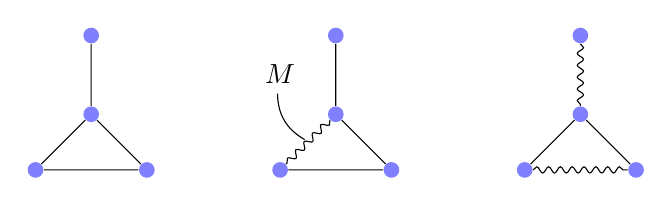
\begin{tikzpicture}[>=stealth, node distance=1cm, on grid]
  \tikzstyle{node}=[circle, fill=blue!50, inner sep=2pt]

  \node[node] (1) {};
  \node[node, below=of 1] (2) {};
  \node[node, below left=of 2] (3) {};
  \node[node, below right=of 2] (4) {};

  \draw (1) -- (2) -- (3) -- (4) -- (2);


  \node[node, right=3cm] at (1) (2-1) {};
  \node[node, below=of 2-1] (2-2) {};
  \node[node, below left=of 2-2] (2-3) {};
  \node[node, below right=of 2-2] (2-4) {};

  \draw (2-1) -- (2-2) -- (2-4) -- (2-3);
  \draw[match] (2-2) -- node[inner sep=1pt] (mid) {} (2-3);

  \node[above left=of 2-2,yshift=-.2cm] (m) {$M$};
  \draw (m) to[->, bend right] (mid);


  \node[node, right=3cm] at (2-1) (3-1) {};
  \node[node, below=of 3-1] (3-2) {};
  \node[node, below left=of 3-2] (3-3) {};
  \node[node, below right=of 3-2] (3-4) {};

  \draw (3-2) -- (3-3);
  \draw (3-2) -- (3-4);
  \draw[match] (3-1) -- (3-2);
  \draw[match] (3-3) -- (3-4);
\end{tikzpicture}
  \end{center}
\end{frame}

\begin{frame} \frametitle{Augmenting Paths}
  \begin{itemize}
  \item An \blue{alternating path} in $(G, M)$ is a simple path whose
    edges are alternately in $M$ and not in $M$.
  \item An \blue{augmenting path} is an alternating path whose ends
    are distinct exposed vertices.
  \end{itemize}
  \begin{center}
    \hfill
    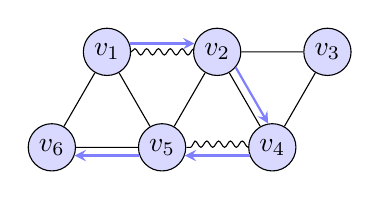
\begin{tikzpicture}[>=stealth, on grid, node distance=1.4cm]
  \node[node]                    (v1) {$v_1$};
  \node[node, right=of v1]       (v2) {$v_2$};
  \node[node, right=of v2]       (v3) {$v_3$};
  \draw (v3) ++(240:1.4cm) node[node]  (v4) {$v_4$};
  \node[node, left=of v4]        (v5) {$v_5$};
  \node[node, left=of v5]        (v6) {$v_6$};

  \draw[match] (v1) -- (v2) (v4) -- (v5);
  \draw (v2) -- (v3) -- (v4) (v5) -- (v6) -- (v1) -- (v5) --
  (v2) -- (v4);

  \draw[path] (v1.20) -- (v2.160);
  \draw[path] (v2.-40) -- (v4.100);
  \draw[path] (v4.200) -- (v5.-20);
  \draw[path] (v5.200) -- (v6.-20);
\end{tikzpicture}%
    \hfill
    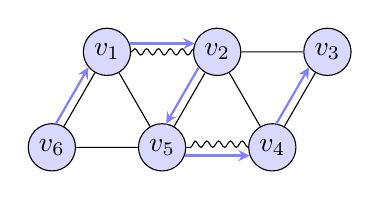
\begin{tikzpicture}[>=stealth, on grid, node distance=1.4cm]
  \node[node]                    (v1) {$v_1$};
  \node[node, right=of v1]       (v2) {$v_2$};
  \node[node, right=of v2]       (v3) {$v_3$};
  \draw (v3) ++(240:1.4cm) node[node]  (v4) {$v_4$};
  \node[node, left=of v4]        (v5) {$v_5$};
  \node[node, left=of v5]        (v6) {$v_6$};

  \draw[match] (v1) -- (v2) (v4) -- (v5);
  \draw (v2) -- (v3) -- (v4) (v5) -- (v6) -- (v1) -- (v5) --
  (v2) -- (v4);

  \draw[path] (v6.80) -- (v1.220);
  \draw[path] (v1.20) -- (v2.160);
  \draw[path] (v2.220) -- (v5.80);
  \draw[path] (v5.-20) -- (v4.-160);
  \draw[path] (v4.80) -- (v3.220);
\end{tikzpicture}%
    \hfill~
  \end{center}
\end{frame}

\subsection{Berge's Theorem}

\begin{frame} \frametitle{Berge's Theorem}
  \begin{block}{Berge's Theorem (1957)}
    A matched graph $(G, M)$ has an augmenting path if and only if $M$
    is not maximum.
  \end{block}
  \begin{columns}[T]
    \begin{column}{.5\textwidth}
      \centering 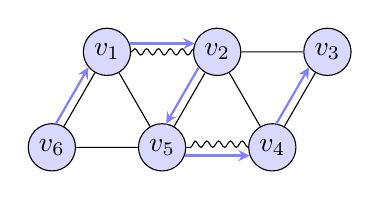
\begin{tikzpicture}[>=stealth, on grid, node distance=1.4cm]
  \node[node]                    (v1) {$v_1$};
  \node[node, right=of v1]       (v2) {$v_2$};
  \node[node, right=of v2]       (v3) {$v_3$};
  \draw (v3) ++(240:1.4cm) node[node]  (v4) {$v_4$};
  \node[node, left=of v4]        (v5) {$v_5$};
  \node[node, left=of v5]        (v6) {$v_6$};

  \draw[match] (v1) -- (v2) (v4) -- (v5);
  \draw (v2) -- (v3) -- (v4) (v5) -- (v6) -- (v1) -- (v5) --
  (v2) -- (v4);

  \draw[path] (v6.80) -- (v1.220);
  \draw[path] (v1.20) -- (v2.160);
  \draw[path] (v2.220) -- (v5.80);
  \draw[path] (v5.-20) -- (v4.-160);
  \draw[path] (v4.80) -- (v3.220);
\end{tikzpicture}\\[4ex]
    \end{column}
    \begin{column}{.5\textwidth}
      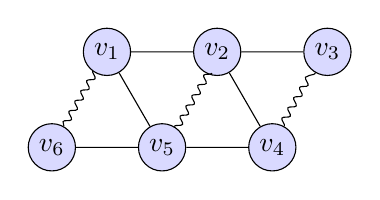
\begin{tikzpicture}[>=stealth, on grid, node distance=1.4cm]
  \node[node]                    (v1) {$v_1$};
  \node[node, right=of v1]       (v2) {$v_2$};
  \node[node, right=of v2]       (v3) {$v_3$};
  \draw (v3) ++(240:1.4cm) node[node]  (v4) {$v_4$};
  \node[node, left=of v4]        (v5) {$v_5$};
  \node[node, left=of v5]        (v6) {$v_6$};

  \draw[match] (v6) -- (v1) (v5) -- (v2) (v4) -- (v3);
  \draw (v1) -- (v2) -- (v3) (v4) -- (v5) -- (v6) (v1) -- (v5) (v2) -- (v4);

%   \draw[path] (v6.80) -- (v1.220);
%   \draw[path] (v1.20) -- (v2.160);
%   \draw[path] (v2.220) -- (v5.80);
%   \draw[path] (v5.-20) -- (v4.-160);
%   \draw[path] (v4.80) -- (v3.220);
\end{tikzpicture}\\
      \only<1>{\hfill Unique? \hfill\hfill~}
      % \only<2>{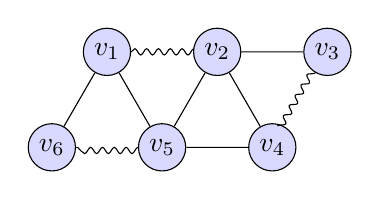
\begin{tikzpicture}[>=stealth, on grid, node distance=1.4cm]
  \node[node]                    (v1) {$v_1$};
  \node[node, right=of v1]       (v2) {$v_2$};
  \node[node, right=of v2]       (v3) {$v_3$};
  \draw (v3) ++(240:1.4cm) node[node]  (v4) {$v_4$};
  \node[node, left=of v4]        (v5) {$v_5$};
  \node[node, left=of v5]        (v6) {$v_6$};

  \draw[match] (v1) -- (v2) (v3) -- (v4) (v5) -- (v6);
  \draw (v2) -- (v3) (v4) -- (v5) (v6) -- (v1) -- (v5) -- (v2) -- (v4);

%   \draw[path] (v6.80) -- (v1.220);
%   \draw[path] (v1.20) -- (v2.160);
%   \draw[path] (v2.220) -- (v5.80);
%   \draw[path] (v5.-20) -- (v4.-160);
%   \draw[path] (v4.80) -- (v3.220);
\end{tikzpicture}}
    \end{column}
  \end{columns}
  \vspace{2ex}
  \textbf{An Exponential Algorithm:}\\
  Exhaustively search for an augmenting path starting from an exposed
  vertex.
\end{frame}

% =============================================================================

\subsection{Bipartite Matching}

\begin{frame} \frametitle{Bipartite Graphs}
  \begin{itemize}
  \item A \blue{bipartite graph} $G=(A, B, E)$ is a graph whose vertices can be
    divided into two disjoint sets $A$ and $B$ such that every
    edge connects a vertex in $A$ to one in $B$.
  \item Equivalently, it is a graph with no odd cycles.
  \end{itemize}
  \begin{center}
    \begin{columns}
      \begin{column}{.5\textwidth}
        \centering 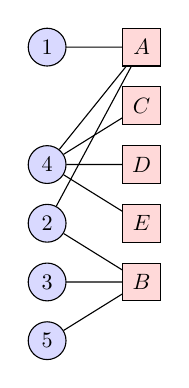
\begin{tikzpicture}[node distance=1.2cm, on grid]
  \tikzstyle{node}+=[scale=.8]
  \tikzstyle{node2}=[node, rectangle, fill=red!15]

  \node[node] (1) {$1$};
  \node[node2, right=of 1] (a) {$A$};
  \node[node2, below=.5cm] at (a) (c) {$C$};
  \node[node2, below=.5cm] at (c) (d) {$D$};
  \node[node2, below=.5cm] at (d) (e) {$E$};
  \node[node2, below=.5cm] at (e) (b) {$B$};
  \node[node, left=of d] (4) {$4$};
  \node[node, left=of b] (3) {$3$};
  \node[node, above=.5cm] at (3) (2) {$2$};
  \node[node, below=.5cm] at (3) (5) {$5$};

  \draw (1) -- (a) -- (2) -- (b) -- (3);
  \draw (a) -- (4) (b) -- (5);
  \draw (c) -- (4) -- (d) (4) -- (e);
\end{tikzpicture}
      \end{column}
      \begin{column}{.5\textwidth}
        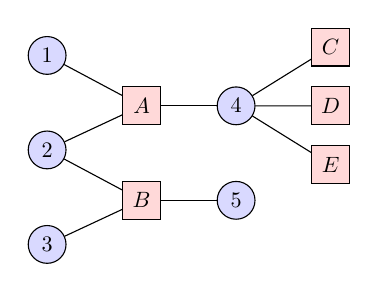
\begin{tikzpicture}[node distance=1.2cm, on grid]
  \tikzstyle{node}+=[scale=.8]
  \tikzstyle{node2}=[node, rectangle, fill=red!15]

  \node[node] (1) {$1$};
  \node[node, below=of 1] (2) {$2$};
  \node[node, below=of 2] (3) {$3$};

  \node[node2, right=of 2, yshift=.7cm] (a) {$A$};
  \node[node2, below=of a] (b) {$B$};

  \node[node, right=of a] (4) {$4$};
  \node[node, right=of b] (5) {$5$};

  \node[node2, right=of 4] (d) {$D$};
  \node[node2, above=.5cm] at (d) (c) {$C$};
  \node[node2, below=.5cm] at (d) (e) {$E$};

  \draw (1) -- (a) -- (2) -- (b) -- (3);
  \draw (a) -- (4) (b) -- (5);
  \draw (c) -- (4) -- (d) (4) -- (e);
\end{tikzpicture}
      \end{column}
    \end{columns}
  \end{center}
\end{frame}

\begin{frame} \frametitle{Bipartite Graph Maximum Matching}
  \vspace{-1ex}
  \begin{columns}[b]
    \begin{column}{.15\textwidth}
      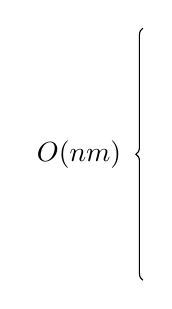
\begin{tikzpicture}
        \draw[decorate, decoration=brace] (0,0) -- node[left=1ex] {$O(nm)$} (0,3.2);
      \end{tikzpicture}
    \end{column}
    \begin{column}{.9\textwidth}
      \begin{algorithmic}
        \FORALL {$v \in A$, $v$ is exposed}
        \STATE Search for simple alternating paths starting at $v$
        \IF {path $P$ ends at an exposed vertex $u \in B$}
        \STATE $P$ is an augmenting path
        \COMMENT {Update $M$}
        \ENDIF
        \ENDFOR
        \STATE Current $M$ is maximum \COMMENT {No more augmenting
          paths}
      \end{algorithmic}
    \end{column}
  \end{columns}
  % \begin{itemize}
  % \item Can be improved to $O(m \sqrt{n})$.
  % \end{itemize}
  \vspace{1ex}
  \begin{columns}
    \begin{column}{.5\textwidth}
      \centering 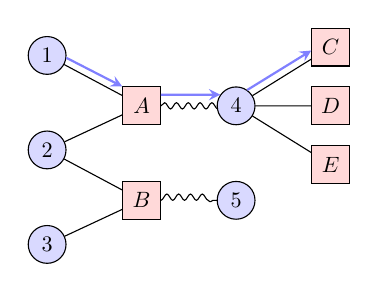
\begin{tikzpicture}[>=stealth, node distance=1.2cm, on grid]
  \tikzstyle{node}+=[scale=.8]
  \tikzstyle{node2}=[node, rectangle, fill=red!15]

  \node[node] (1) {$1$};
  \node[node, below=of 1] (2) {$2$};
  \node[node, below=of 2] (3) {$3$};

  \node[node2, right=of 2, yshift=.7cm] (a) {$A$};
  \node[node2, below=of a] (b) {$B$};

  \node[node, right=of a] (4) {$4$};
  \node[node, right=of b] (5) {$5$};

  \node[node2, right=of 4] (d) {$D$};
  \node[node2, above=.5cm] at (d) (c) {$C$};
  \node[node2, below=.5cm] at (d) (e) {$E$};

  \draw (1) -- (a) -- (2) -- (b) -- (3);
  \draw[match] (a) -- (4) (b) -- (5);
  \draw (c) -- (4) -- (d) (4) -- (e);

  \draw[path] (1.-7) -- (a.135);
  \draw[path] (a.30) -- (4.145);
  \draw[path] (4.55) -- (c.190);
\end{tikzpicture}
    \end{column}
    \begin{column}{.5\textwidth}
      \uncover<2>{
        \centering 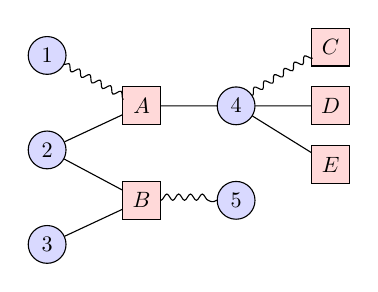
\begin{tikzpicture}[>=stealth, node distance=1.2cm, on grid]
  \tikzstyle{node}+=[scale=.8]
  \tikzstyle{node2}=[node, rectangle, fill=red!15]

  \node[node] (1) {$1$};
  \node[node, below=of 1] (2) {$2$};
  \node[node, below=of 2] (3) {$3$};

  \node[node2, right=of 2, yshift=.7cm] (a) {$A$};
  \node[node2, below=of a] (b) {$B$};

  \node[node, right=of a] (4) {$4$};
  \node[node, right=of b] (5) {$5$};

  \node[node2, right=of 4] (d) {$D$};
  \node[node2, above=.5cm] at (d) (c) {$C$};
  \node[node2, below=.5cm] at (d) (e) {$E$};

  \draw (a) -- (2) -- (b) -- (3);
  \draw[match] (1) -- (a) (4) -- (c) (b) -- (5);
  \draw (a) -- (4) -- (d) (4) -- (e);
\end{tikzpicture}}
    \end{column}
  \end{columns}
\end{frame}

\begin{frame} \frametitle{Non-Bipartite Matching}
  \textbf{Problem:} Odd cycles \ldots
  \begin{center}
    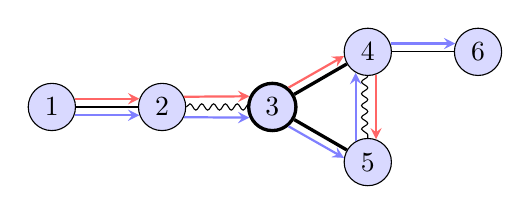
\begin{tikzpicture}[>=stealth, node distance=1.4cm, on grid]
%  \tikzstyle{node}+=[scale=.8]

  \node[node] (1) {$1$};
  \node[node, right=of 1] (2) {$2$};
  \node[node, very thick, right=of 2] (3) {$3$};
  \draw (3) ++(30:1.4cm) node[node] (4) {$4$};
  \node[node, below=of 4] (5) {$5$};
  \node[node, right=of 4] (6) {$6$};

  \draw (1) -- (2) (4) -- (6);
  \draw[very thick] (3) -- (4) (3) -- (5);
  \draw[match] (2) -- (3) (4) -- (5);

  \draw[path,red!60] (1.20) -- (2.160);
  \draw[path,red!60] (2.25) -- (3.155);
  \draw[path,red!60] (3.50) -- (4.190);
  \draw[path,red!60] (4.-70) -- (5.70);

  \draw[path] (1.-20) -- (2.-160);
  \draw[path] (2.-25) -- (3.-155);
  \draw[path] (3.-50) -- (5.170);
  \draw[path] (5.120) -- (4.-120);
  \draw[path] (4.20) -- (6.160);
\end{tikzpicture}\\
    \vspace{1cm}
    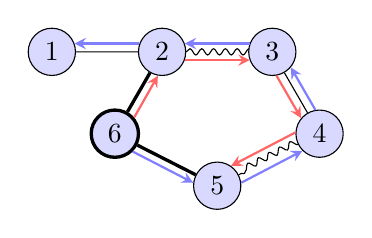
\begin{tikzpicture}[>=stealth, node distance=1.4cm, on grid]
%  \tikzstyle{node}+=[scale=.8]

  \node[node] (1) {$1$};
  \node[node, right=of 1] (2) {$2$};
  \node[node, right=of 2] (3) {$3$};
  \draw (3) ++(-60:1.2cm) node[node] (4) {$4$};
  \draw (2) ++(240:1.2cm) node[node, very thick] (6) {$6$};
  \draw (2) ++(.7cm,-1.7cm) node[node] (5) {$5$};

  \draw (1) -- (2) (3) -- (4);
  \draw[very thick] (2) -- (6) -- (5);
  \draw[match] (2) -- (3) (4) -- (5);

  \draw[path,red!60] (6.40) -- (2.-100);
  \draw[path,red!60] (2.-20) -- (3.-160);
  \draw[path,red!60] (3.-80) -- (4.140);
  \draw[path,red!60] (4.177) -- (5.55);

  \draw[path] (6.-45) -- (5.173);
  \draw[path] (5.7) -- (4.-135);
  \draw[path] (4.100) -- (3.-40);
  \draw[path] (3.160) -- (2.20);
  \draw[path] (2.160) -- (1.20);

\end{tikzpicture}
  \end{center}
\end{frame}

% =============================================================================

%\section{Edmonds' Algorithm}

\section{Paths, Trees and Flowers}

\subsection{Blossoms}

\begin{frame} \frametitle{Blossoms}
  \begin{block}{Blossoms}
    A blossom $B$ in $(G, M)$ is an odd cycle with a unique exposed
    vertex (the base) in $M \cap B$.
  \end{block}
  \begin{center}
    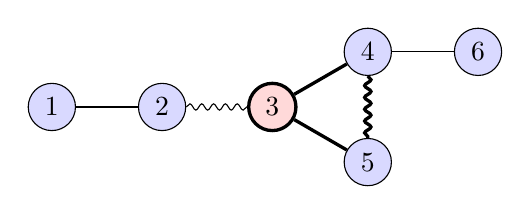
\begin{tikzpicture}[>=stealth, node distance=1.4cm, on grid]
%  \tikzstyle{node}+=[scale=.8]

  \node[node] (1) {$1$};
  \node[node, right=of 1] (2) {$2$};
  \node[node, very thick, fill=red!15, right=of 2] (3) {$3$};
  \draw (3) ++(30:1.4cm) node[node] (4) {$4$};
  \node[node, below=of 4] (5) {$5$};
  \node[node, right=of 4] (6) {$6$};

  \draw (1) -- (2) (4) -- (6);
  \draw[very thick] (3) -- (4) (3) -- (5);
  \draw[match] (2) -- (3);
  \draw[match, very thick] (4) -- (5);
\end{tikzpicture}\\
    \vspace{.5cm}
    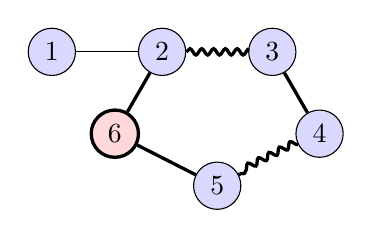
\begin{tikzpicture}[>=stealth, node distance=1.4cm, on grid]
%  \tikzstyle{node}+=[scale=.8]

  \node[node] (1) {$1$};
  \node[node, right=of 1] (2) {$2$};
  \node[node, right=of 2] (3) {$3$};
  \draw (3) ++(-60:1.2cm) node[node] (4) {$4$};
  \draw (2) ++(240:1.2cm) node[node, very thick, fill=red!15] (6) {$6$};
  \draw (2) ++(.7cm,-1.7cm) node[node] (5) {$5$};

  \draw (1) -- (2);
  \draw[very thick] (2) -- (6) -- (5) (3) -- (4);
  \draw[match, very thick] (2) -- (3) (4) -- (5);
\end{tikzpicture}
  \end{center}
\end{frame}

\begin{frame} \frametitle{Edmonds' Blossoms Lemma}
  \begin{block}{Blossoms Lemma}
    Let $G'$ and $M'$ be obtained by contracting a blossom $B$ in $(G,
    M)$ to a single vertex.\\
    The matching $M$ of $G$ is maximum iff $M'$ is maximum in $G'$.
  \end{block}
  \begin{center}
    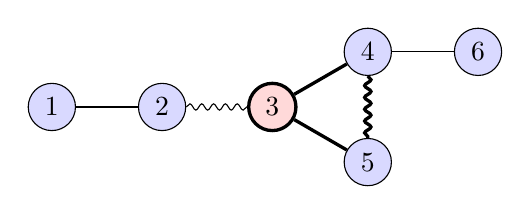
\begin{tikzpicture}[>=stealth, node distance=1.4cm, on grid]
%  \tikzstyle{node}+=[scale=.8]

  \node[node] (1) {$1$};
  \node[node, right=of 1] (2) {$2$};
  \node[node, very thick, fill=red!15, right=of 2] (3) {$3$};
  \draw (3) ++(30:1.4cm) node[node] (4) {$4$};
  \node[node, below=of 4] (5) {$5$};
  \node[node, right=of 4] (6) {$6$};

  \draw (1) -- (2) (4) -- (6);
  \draw[very thick] (3) -- (4) (3) -- (5);
  \draw[match] (2) -- (3);
  \draw[match, very thick] (4) -- (5);
\end{tikzpicture}\\
    \vspace{.5cm}
    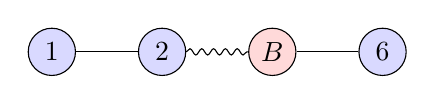
\begin{tikzpicture}[>=stealth, node distance=1.4cm, on grid]
%  \tikzstyle{node}+=[scale=.8]

  \node[node] (1) {$1$};
  \node[node, right=of 1] (2) {$2$};

%  \node[node, very thick, fill=red!15, right=of 2] (3) {$3$};
%  \draw (3) ++(30:1.4cm) node[node] (4) {$4$};
%  \node[node, below=of 4] (5) {$5$};
  \node[node, fill=red!15, right=of 2] (b) {$B$};

  \node[node, right=of b] (6) {$6$};

  \draw (1) -- (2) (b) -- (6);
%  \draw[very thick] (3) -- (4) (3) -- (5);
  \draw[match] (2) -- (b);
%  \draw[match, very thick] (4) -- (5);
\end{tikzpicture}
  \end{center}
\end{frame}

\begin{frame} \frametitle{Detecting Blossoms}
  \begin{itemize}
  \item Performing the alternating path search of the bipartite
    matching algorithm (starting from an exposed vertex):
    \begin{itemize}
    \item[\subbullet] Label vertices at even distance from the root as
      ``\blue{outer}'';
    \item[\subbullet] Label vertices at odd distance from the root as
      ``\blue{inner}''.
    \end{itemize}
  \item If two outer vertices are found adjacent, we have a blossom.
  \end{itemize}
  \begin{center}
    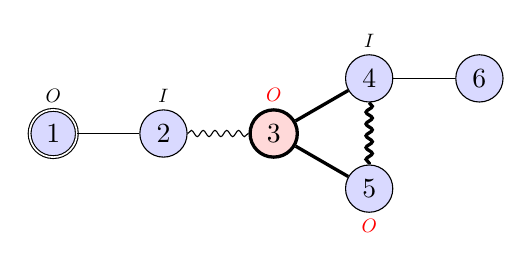
\begin{tikzpicture}[>=stealth, node distance=1.4cm, on grid]
  \tikzstyle{lbl}=[scale=.7, anchor=south]

  \node[node, double] (1) {$1$};
  \node[node, right=of 1] (2) {$2$};
  \node[node, very thick, fill=red!15, right=of 2] (3) {$3$};
  \draw (3) ++(30:1.4cm) node[node] (4) {$4$};
  \node[node, below=of 4] (5) {$5$};
  \node[node, right=of 4] (6) {$6$};

  \node[lbl] at (1.north) {$O$};
  \node[lbl] at (2.north) {$I$};
  \node[lbl,red] at (3.north) {$O$};
  \node[lbl] at (4.north) {$I$};
  \node[lbl,red,anchor=north] at (5.south) {$O$};

  \draw (1) -- (2) (4) -- (6);
  \draw[very thick] (3) -- (4) (3) -- (5);
  \draw[match] (2) -- (3);
  \draw[match, very thick] (4) -- (5);
\end{tikzpicture}
  \end{center}
\end{frame}

\subsection{The Algorithm}

\begin{frame} \frametitle{Edmonds' Algorithm (1965)}
  \vspace{-2ex}
  \begin{columns}[T]
    \begin{column}{.1\textwidth}
      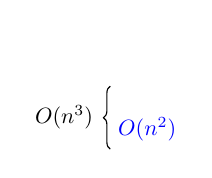
\begin{tikzpicture}[every node/.style={scale=.8}]
        \node at (0,1.2cm) {};
        \node[blue] (b) {$O(n^2)$};
        \draw[decorate,decoration=brace] (b.south west) -- node[left=.8ex]
        {$O(n^3)$} ++(0,.8cm);
      \end{tikzpicture}
    \end{column}
    \begin{column}{.9\textwidth}
      \begin{algorithmic}
        \FORALL {$v \in V$, $v$ is exposed}
        \STATE Search for simple alternating paths starting at $v$
        \STATE \hspace{2ex} \blue{Shrink any found blossoms}
        \IF {path $P$ ends at an exposed vertex}
        \STATE $P$ is an augmenting path
        \COMMENT {Update $M$}
        \ELSIF {\blue{no augmenting paths found}}
        \STATE \blue{Ignore $v$ in future searches}
        \ENDIF
        \ENDFOR
        \STATE Current $M$ is maximum \COMMENT {No more augmenting
          paths}
      \end{algorithmic}
    \end{column}
  \end{columns}
  \vspace{.5cm}

  \begin{columns}
    \begin{column}{.4\textwidth}
      \begin{block}{}
        \centering \textbf{Complexity:} $O(n^4)$
      \end{block}
    \end{column}
  \end{columns}

\end{frame}

\begin{frame} \frametitle{Example}
  $\textcolor<8>{black!30}{|M| = 4}$ \hfill \uncover<8>{\blue{$|M|=5$}}
  \begin{center}
    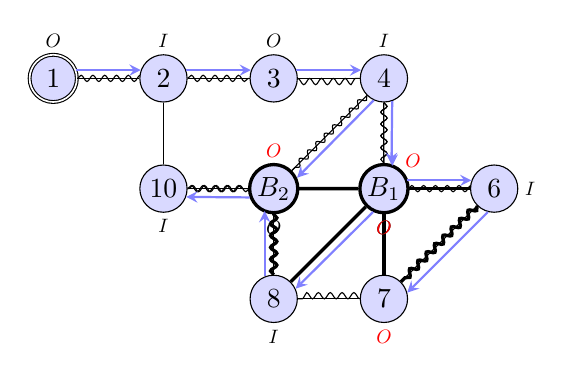
\begin{tikzpicture}[>=stealth, node distance=1.4cm, on grid]
  \tikzstyle{lbl}=[scale=.7, anchor=south]

%%%%%%%%%%%%%%%% Nodes %%%%%%%%%%%%%%%%

  \node[node, double] (1) {$1$};
  \node[node, right=of 1] (2) {$2$};
  \node[node, right=of 2] (3) {$3$};
  \node[node, right=of 3] (4) {$4$};
  \node[node, below=of 2] (10) {$10$};
  \uncover<1-4,7->{
    \node[node, right=of 10] (9) {$9$};
    \node[node, below=of 9] (8) {$8$};
  }
  \uncover<1-2,8>{
    \node[node, right=of 9] (5) {$5$};
    \node[node, right=of 5] (6) {$6$};
    \node[node, right=of 8] (7) {$7$};
  }
  \uncover<3-4,7>{
    \node[node, very thick, right=of 9] (b1) {$B_1$};
  }
  \uncover<5-6>{
    \node[node, very thick, right=of 10] (b2) {$B_2$};
  }

%%%%%%%%%%%%%%%% Edges %%%%%%%%%%%%%%%%

  \uncover<1-5>{
    \draw (1) -- (2) (3) -- (4) (10) -- (2);
    \draw[match] (2) -- (3);
  }

  \uncover<1>{
    \draw[match] (6) -- (7);
    \draw (6) -- (5) -- (7);
  }

  \uncover<1-2>{
    \draw[match] (4) -- (5);
    \draw (5) -- (9) (7) -- (8);
  }

  \uncover<1-3>{
    \draw[match] (8) -- (9);
  }

  \uncover<1-4>{
    \draw (9) -- (10);
  }

  \uncover<2>{
    \draw[match, very thick] (6) -- (7);
    \draw[very thick] (6) -- (5) -- (7);
  }

  \uncover<3-4>{
    \draw[match] (4) -- (b1);
  }

  \uncover<3,7>{
    \draw (9) -- (b1) -- (8);
  }

  \uncover<4>{
    \draw[match, very thick] (8) -- (9);
    \draw[very thick] (9) -- (b1) -- (8);
  }

  \uncover<5>{
    \draw[match] (4) -- (b2);
    \draw (b2) -- (10);
  }

  \uncover<6>{
    \draw[match] (10) -- (b2);
    \draw (4) -- (b2);
  }

  \uncover<6->{
    \draw[match] (1) -- (2) (3) -- (4);
    \draw (2) -- (3) (10) -- (2);
  }

  \uncover<7>{
    \draw (4) -- (b1);
  }

  \uncover<7->{
    \draw[match] (9) -- (10);
    \draw (8) -- (9);
  }

  \uncover<8>{
    \draw[match] (5) -- (6) (7) -- (8);
    \draw (6) -- (7) -- (5) -- (9) (4) -- (5);
  }

%%%%%%%%%%%%%%%% Paths %%%%%%%%%%%%%%%%

  \uncover<2-5>{
    \draw[path] (1.20) -- (2.160);
    \draw[path] (2.20) -- (3.160);
    \draw[path] (3.20) -- (4.160);
  }

  \uncover<2>{
    \draw[path] (4.-70) -- (5.70);
    \draw[path] (5.20) -- (6.160);
    \draw[path] (6.-105) -- (7.15);
  }

  \uncover<3-4>{
    \draw[path] (4.-70) -- (b1.73);
  }

  \uncover<4>{
    \draw[path] (b1.-115) -- (8.25);
    \draw[path] (8.112) -- (9.-112);
  }

  \uncover<5>{
    \draw[path] (4.-115) -- (b2.25);
    \draw[path] (b2.-160) -- (10.-20);
  }

%%%%%%%%%%%%%%%% Labels %%%%%%%%%%%%%%%%

  \uncover<2-5>{
    \node[lbl] at (1.north) {$O$};
    \node[lbl] at (2.north) {$I$};
    \node[lbl] at (3.north) {$O$};
    \node[lbl] at (4.north) {$I$};
  }

  \uncover<2>{
    \node[lbl,red,anchor=south west, inner sep=2pt] at (5.north east) {$O$};
    \node[lbl,anchor=west] at (6.east) {$I$};
    \node[lbl,red,anchor=north] at (7.south) {$O$};
  }

  \uncover<3>{
    \node[lbl,anchor=north] at (b1.south) {$O$};
  }

  \uncover<4>{
    \node[lbl,anchor=north,red] at (b1.south) {$O$};
    \node[lbl,anchor=north] at (8.south) {$I$};
    \node[lbl,anchor=south,red] at (9.north) {$O$};
  }

  \uncover<5>{
    \node[lbl,anchor=north] at (b2.south) {$O$};
    \node[lbl,anchor=north] at (10.south) {$I$};
  }
\end{tikzpicture}
  \end{center}
  \uncover<3->{$B_1 = 5, 6, 7$}\\
  \uncover<5->{$B_2 = B_1, 8, 9 = 5, 6, 7, 8, 9$}
\end{frame}

% =============================================================================

%\section[Gabow's Implementation]{Efficient Implementation of Edmonds' Algorithm}
\section[Efficient Implementation]{Efficient Implementation of Edmonds'
  Algorithm}

\subsection{Data Structures}

\begin{frame} \frametitle{Three Arrays}
  \vspace{-2ex}
  \begin{itemize}
  \item $\blue{u}$ is an exposed vertex.
  \item A vertex $\blue{v}$ is \blue{outer} if there is a path $P(\blue{v}) = (\blue{v},
    v_1, \ldots, \blue{u})$, where $vv_1 \in M$.
  \end{itemize}
  \begin{enumerate}
  \item \emph{\textrm{MATE:}} Specifies a matching. An entry for each vertex:
    \begin{itemize}
    \item[\subbullet] $vw \in M \Rightarrow \mathit{MATE}(v) = w$ and $\mathit{MATE}(w) = v$.
    \end{itemize}
  \item \emph{\textrm{LABEL:}} Provides a type and a value:%
    \vspace{-2ex}
    \[%
    \renewcommand{\arraycolsep}{.5ex}
    \begin{array}{rll}
      & \mathit{LABEL}(v) \ge 0 & \rightarrow \; v \text{ is outer} \\
      & \mathit{LABEL}(\blue{u}) & \rightarrow \; \text{\blue{start} label, } P(u)
      = (u)\\
      1 \le & \mathit{LABEL}(v) \le n & \rightarrow \;
      \text{\blue{vertex} label}\\
      n+1 \le & \mathit{LABEL}(v) \le n+2m
      & \rightarrow \; \text{\blue{edge} label}
    \end{array}
    \]
  \item $\mathit{START}(v)$ = the first non-outer vertex
      in $P(v)$.
  \end{enumerate}
\end{frame}

\subsection{The Algorithm}

\begin{frame} \frametitle{Gabow's Algorithm (1976)}
  \vspace{-2ex}
  \begin{columns}
    \begin{column}{.05\textwidth}
      \uncover<2>{
      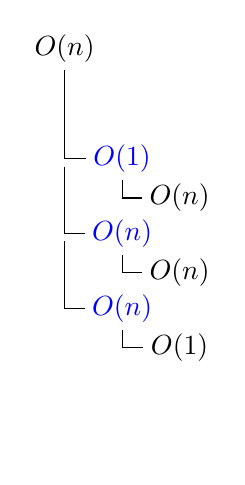
\begin{tikzpicture}[every node/.style={inner sep=2.5pt}]
        \node at (-0.73cm,0) (for) {$O(n)$};

        \node[blue] at (0,-1.4cm) (if) {$O(1)$};
        \node at (0.73,-1.9cm) (aug) {$O(n)$};

        \node[blue] at (0,-2.35cm) (else1) {$O(n)$};
        \node at (0.73,-2.85cm) (edge) {$O(n)$};

        \node[blue] at (0,-3.3cm) (else2) {$O(n)$};
        \node at (0.73,-3.8cm) (vertex) {$O(1)$};

        \node at (-.8cm,-5.1cm) {};

        \draw (if) |- (aug);
        \draw (else1) |- (edge);
        \draw (else2) |- (vertex);
        \draw (for) |- (if);
        \draw (for |- if) ++(0,-.1cm) |- (else1);
        \draw (for |- else1) ++(0,-.1cm) |- (else2);
      \end{tikzpicture}}
    \end{column}
    \begin{column}{.85\textwidth}
      \begin{algorithmic}
        \FORALL {$u \in V, u$ is exposed}
        \color<2>{blue}\WHILE {\color{black}$\exists$ an edge $xy$, $x$ is outer AND\\
          \hspace{.9cm} no augmenting path found}
        \IF {$y$ is exposed, $y \ne u$}
        \STATE $(y, x, \ldots, u)$ is an augmenting path
        \ELSIF {$y$ is outer}
        \STATE Assign edge labels to $P(x)$ and
        $P(y)$
        \ELSIF {$\mathit{MATE}(y)$ is non-outer}
        \STATE Assign a vertex label to $\mathit{MATE}(y)$
        \ENDIF
        \ENDWHILE
        \ENDFOR
      \end{algorithmic}
    \end{column}
  \end{columns}

  \begin{columns}
    \begin{column}{.4\textwidth}
      \uncover<2>{
      \begin{block}{}
        \centering \textbf{Complexity:} $O(n^3)$
      \end{block}}
    \end{column}
  \end{columns}

\end{frame}

\subsection{Performance}

\begin{frame} \frametitle{Experimental Performance}
  Using an implementation in Algol W on the IBM 360/165
  \begin{itemize}
  \item Worst-case graphs:
    \begin{itemize}
    \item[\subbullet] Efficient Implementation: run times proportional to $n^{2.8}$.
    \item[\subbullet] Edmond: run times proportional to $n^{3.5}$.
    \end{itemize}

  \item Random graphs: times one order of magnitude faster than
    worst-case graphs.
  \item Space used is $5n + 4m$.
  \end{itemize}
\end{frame}

% =============================================================================

%\section[Blum's Algorithm]{Reachability Problem Approach}
\section[Reachability Approach]{Reachability Problem Approach}

\subsection{Reachability and Graphs}

\begin{frame} \frametitle{The Reachability Problem in Bipartite
    Graphs}
  \vspace{-1.5ex}
  \begin{itemize}
  \item Construction:
    \vspace{-2ex}
    \[
    \begin{array} {c!{+}c!{\rightarrow}c}
      \text{Bipartite graph} & \text{Matching} & \text{Directed graph}\\[-4pt]
      G = (A, B, E) & M & G' = (V', E')
    \end{array}
    \]
    \vspace{-3ex}
    \begin{itemize}
    \item[\subbullet] $V' = V \cup \{\blue{s}, \blue{t}\}$
    \item[\subbullet] $\forall \; \blue{xy \in M}, x \in A, y \in B
      \rightarrow \blue{(x,y)} \in E'$ \qquad {\scriptsize $e \in M
        \Rightarrow e: A \rightarrow B$}
    \item[\subbullet] $\forall \; \blue{xy \notin M}, x \in A, y \in B
      \rightarrow \blue{(y,x)} \in E'$ \qquad {\scriptsize $e \notin M
        \Rightarrow e: B \rightarrow A$}
    \item[\subbullet] $\forall \; b \in B, \blue{b}$ \blue{is exposed}
      $\rightarrow$ add $\blue{(s,b)}$ to $E'$
    \item[\subbullet] $\forall \; a \in A, \blue{a}$ \blue{is exposed}
      $\rightarrow$ add $\blue{(a,t)}$ to $E'$
    \end{itemize}

    \begin{center}
      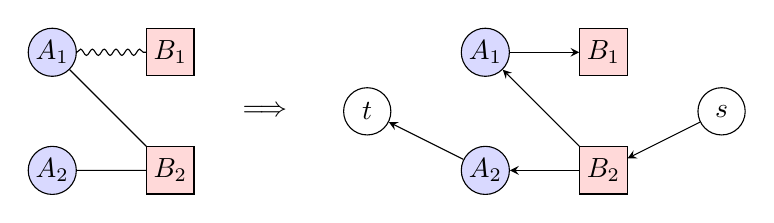
\begin{tikzpicture}[>=stealth, on grid, node distance=1.5cm]
  \node[node] (a1) {$A_1$};
  \node[node, below=of a1] (a2) {$A_2$};
  \node[node2, right=of a1] (b1) {$B_1$};
  \node[node2, below=of b1] (b2) {$B_2$};
  \draw[match] (a1) -- (b1);
  \draw (a1) -- (b2) -- (a2);
  \draw (b2) node[xshift=1.2cm,yshift=.75cm] {$\Longrightarrow$};

  \node[node, right=of b1, xshift=2.5cm] (a1-2) {$A_1$};
  \node[node, below=of a1-2] (a2-2) {$A_2$};
  \node[node2, right=of a1-2] (b1-2) {$B_1$};
  \node[node2, below=of b1-2] (b2-2) {$B_2$};
  \draw (a2-2) node[node, xshift=-1.5cm,yshift=.75cm,fill=white]
  (t) {$t$};
  \draw (b2-2) node[node, xshift=1.5cm,yshift=.75cm,fill=white]
  (s) {$s$};
  \draw[->] (a1-2) -- (b1-2);
  \draw[<-] (a1-2) -- (b2-2);
  \draw[<-] (a2-2) -- (b2-2);
  \draw[->] (s) -- (b2-2);
  \draw[->] (a2-2) -- (t);
\end{tikzpicture}

    \end{center}

  \item<2> An augmenting path in $G$ $\Leftrightarrow$ A simple path
    from $s$ to $t$ in $G'$.
  \end{itemize}
\end{frame}

\begin{frame} \frametitle{The Reachability Problem in General Graphs}
  \framesubtitle{Construction}
  \vspace{-1ex}
  \begin{itemize}
  \item For each $v \in V$, we introduce two nodes $v_A$ and $v_B$
    \[
    V' = \{ v_A, v_B | v \in V\} \cup \{s, t\} \qquad s, t \notin V,
    s \ne t
    \]
  \item $e \in M \Rightarrow e: \blue{A} \rightarrow \alert{B}, \qquad e \notin M
    \Rightarrow e: \alert{B} \rightarrow \blue{A}$
    \[
    \begin{split}
      E' = {} & \hspace{2.5ex} \{ (\blue{x_A}, \alert{y_B}), (\blue{y_A}, \alert{x_B}) \, | \, (x,y) \blue{{}\in{}} M \}\\
              & \cup \{ (\alert{x_B}, \blue{y_A}), (\alert{y_B}, \blue{x_A}) \, | \, (x,y) \blue{{}\notin{}} M \}\\
              & {} \cup \{ (s, \alert{x_B}) \, | \, x \text{ is exposed} \}
              \cup \{ (\blue{x_A}, t) \, | \, x \text{ is exposed} \}
    \end{split}
     \]
  \end{itemize}
  \vspace{-3ex}
  \begin{center}
    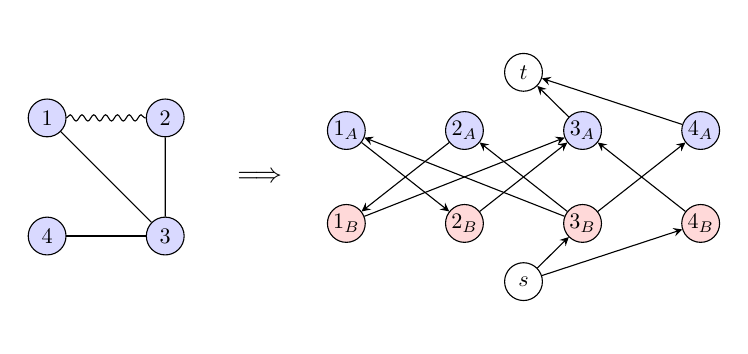
\begin{tikzpicture}[>=stealth, on grid, node distance=1.5cm]
  \tikzstyle{node}+=[scale=.8]
  \tikzstyle{node2}=[node,fill=red!15]

  \node[node] (1) {$1$};
  \node[node, right=of 1] (2) {$2$};
  \node[node, below=of 1] (4) {$4$};
  \node[node, right=of 4] (3) {$3$};

  \draw[match] (1) -- (2);
  \draw (1) -- (3) -- (2);
  \draw (3) -- (4);

  \draw (3) ++(1.2cm,.75cm) node {$\Longrightarrow$};

  \node[node, right=of 2, xshift=1cm,yshift=-.2cm] (1a) {$1_A$};
  \node[node2,below=of 1a, yshift=.4cm] (1b) {$1_B$};
  \node[node, right=of 1a] (2a) {$2_A$};
  \node[node2,right=of 1b] (2b) {$2_B$};
  \node[node, right=of 2a] (3a) {$3_A$};
  \node[node2,right=of 2b] (3b) {$3_B$};
  \node[node, right=of 3a] (4a) {$4_A$};
  \node[node2,right=of 3b] (4b) {$4_B$};

  \draw[->] (1a) -- (2b);
  \draw[->] (2a) -- (1b);
  \draw[->] (2b) -- (3a);
  \draw[->] (3b) -- (2a);
  \draw[->] (3b) -- (4a);
  \draw[->] (4b) -- (3a);
  \draw[->] (1b) -- (3a);
  \draw[->] (3b) -- (1a);

  \draw (2b) ++(-60:1.5cm) node[node,fill=white,yshift=.7cm] (s)
  {$s$};
  \draw (2a) ++(60:1.5cm) node[node,fill=white,yshift=-.7cm] (t)
  {$t$};
  \draw[->] (s) -- (3b);
  \draw[->] (s) -- (4b);
  \draw[->] (3a) -- (t);
  \draw[->] (4a) -- (t);
\end{tikzpicture}

  \end{center}
\end{frame}

\begin{frame} \frametitle{The Reachability Problem in General Graphs}
  \framesubtitle{Strongly Simple Paths}
  A path $P$ in $G'$ is strongly simple if:
  \begin{itemize}
  \item $P$ is simple.
  \item $v_A \in P \Rightarrow v_B \notin P$.
  \end{itemize}
  \begin{block}{Theorem}
    There is an augmenting path in $G$ if and only if there is a
    strongly simple path from $s$ to $t$ in $G'$.
  \end{block}
  \vspace{-2ex}
  \begin{center}
    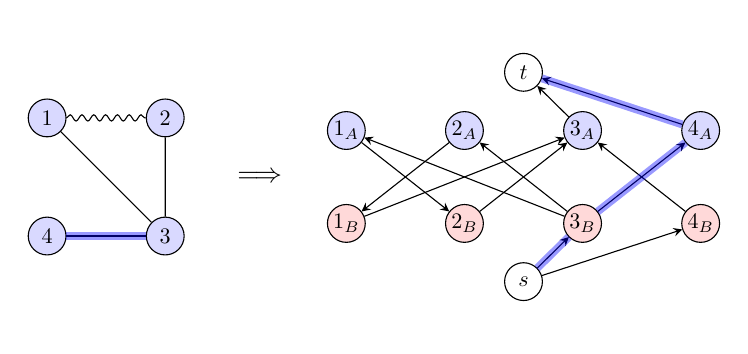
\begin{tikzpicture}[>=stealth, on grid, node distance=1.5cm]
  \tikzstyle{node}+=[scale=.8]
  \tikzstyle{node2}=[node,fill=red!15]

  \node[node] (1) {$1$};
  \node[node, right=of 1] (2) {$2$};
  \node[node, below=of 1] (4) {$4$};
  \node[node, right=of 4] (3) {$3$};

  \draw[match] (1) -- (2);
  \draw (1) -- (3) -- (2);
  \draw (3) -- (4);

  \draw (3) ++(1.2cm,.75cm) node {$\Longrightarrow$};

  \node[node, right=of 2, xshift=1cm,yshift=-.2cm] (1a) {$1_A$};
  \node[node2,below=of 1a, yshift=.4cm] (1b) {$1_B$};
  \node[node, right=of 1a] (2a) {$2_A$};
  \node[node2,right=of 1b] (2b) {$2_B$};
  \node[node, right=of 2a] (3a) {$3_A$};
  \node[node2,right=of 2b] (3b) {$3_B$};
  \node[node, right=of 3a] (4a) {$4_A$};
  \node[node2,right=of 3b] (4b) {$4_B$};

  \draw[->] (1a) -- (2b);
  \draw[->] (2a) -- (1b);
  \draw[->] (2b) -- (3a);
  \draw[->] (3b) -- (2a);
  \draw[->] (3b) -- (4a);
  \draw[->] (4b) -- (3a);
  \draw[->] (1b) -- (3a);
  \draw[->] (3b) -- (1a);

  \draw (2b) ++(-60:1.5cm) node[node,fill=white,yshift=.7cm] (s)
  {$s$};
  \draw (2a) ++(60:1.5cm) node[node,fill=white,yshift=-.7cm] (t)
  {$t$};
  \draw[->] (s) -- (3b);
  \draw[->] (s) -- (4b);
  \draw[->] (3a) -- (t);
  \draw[->] (4a) -- (t);

  \draw[blue,opacity=.4,line width=1mm] (s) -- (3b) -- (4a) -- (t);
  \draw[blue,opacity=.4,line width=1mm] (3) -- (4);
\end{tikzpicture}

  \end{center}
\end{frame}

\begin{frame} \frametitle{Solving the Reachability Problem}
  \textbf{Solution:} A strongly simple path from $s$ to $t$ in $G'$:
  \begin{itemize}
  \item Depth-First Search (DFS) for $t$ starting at $s$.
  \item DFS finds simple paths.
  \item We need to find strongly simple paths only.
  \item We use a Modified Depth-First Search (MDFS) algorithm.
  \end{itemize}

  \vspace{1ex}
  \textbf{Example:}
  \vspace{-1ex}
  \begin{center}
    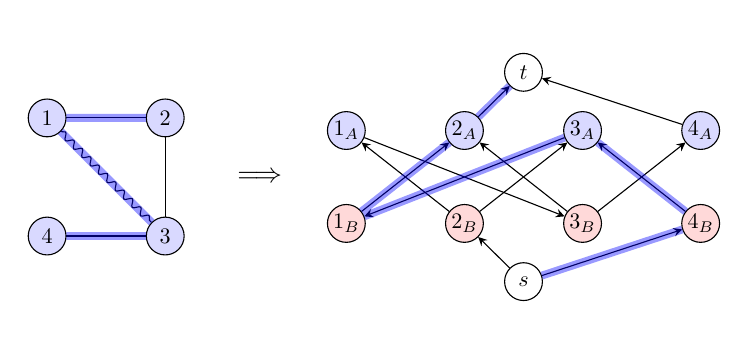
\begin{tikzpicture}[>=stealth, on grid, node distance=1.5cm]
  \tikzstyle{node}+=[scale=.8]
  \tikzstyle{node2}=[node,fill=red!15]

  \node[node] (1) {$1$};
  \node[node, right=of 1] (2) {$2$};
  \node[node, below=of 1] (4) {$4$};
  \node[node, right=of 4] (3) {$3$};

  \draw[match] (1) -- (3);
  \draw (1) -- (2) -- (3);
  \draw (3) -- (4);

  \draw (3) ++(1.2cm,.75cm) node {$\Longrightarrow$};

  \node[node, right=of 2, xshift=1cm,yshift=-.2cm] (1a) {$1_A$};
  \node[node2,below=of 1a, yshift=.4cm] (1b) {$1_B$};
  \node[node, right=of 1a] (2a) {$2_A$};
  \node[node2,right=of 1b] (2b) {$2_B$};
  \node[node, right=of 2a] (3a) {$3_A$};
  \node[node2,right=of 2b] (3b) {$3_B$};
  \node[node, right=of 3a] (4a) {$4_A$};
  \node[node2,right=of 3b] (4b) {$4_B$};

  \draw[->] (1b) -- (2a);
  \draw[->] (2b) -- (1a);
  \draw[->] (2b) -- (3a);
  \draw[->] (3b) -- (2a);
  \draw[->] (3b) -- (4a);
  \draw[->] (4b) -- (3a);
  \draw[->] (1a) -- (3b);
  \draw[->] (3a) -- (1b);

  \draw (2b) ++(-60:1.5cm) node[node,fill=white,yshift=.7cm] (s)
  {$s$};
  \draw (2a) ++(60:1.5cm) node[node,fill=white,yshift=-.7cm] (t)
  {$t$};
  \draw[->] (s) -- (2b);
  \draw[->] (s) -- (4b);
  \draw[->] (2a) -- (t);
  \draw[->] (4a) -- (t);

  \uncover<2>{
    \draw[blue,opacity=.4,line width=1mm] (s) -- (4b) -- (3a) -- (1b)
    -- (2a) -- (t);
    \draw[blue,opacity=.4,line width=1mm] (4) -- (3) -- (1) -- (2);
  }
\end{tikzpicture}

  \end{center}
\end{frame}

\subsection{The Algorithm}

\begin{frame} \frametitle{Data Structures}
  \begin{itemize}
  \item Stack $K$
    \begin{itemize}
    \item[\subbullet] \textrm{TOP($K$)}: the last vertex added to the stack $K$.
    \item[\subbullet] Vertices in $K$ form the current path.
    \item[\subbullet] In each step, the MDFS algorithm considers an
      edge \textrm{(TOP($K$), $v$)}, $v \in V'$.
    \end{itemize}
    \vspace{3ex}
  \item List $L(v_A)$
    \begin{itemize}
    \item[\subbullet] To get a strongly simple path, $v_A$ and $v_B$
      cannot be in $K$ simultaneously (we may ignore a vertex,
      \emph{temporarily}).
    \item[\subbullet] List $L(v_A)$ keeps track of such vertices.
    \end{itemize}
  \end{itemize}
\end{frame}

\begin{frame} \frametitle{Hopcroft and Karp Algorithm for Bipartite
    Graphs (1973)}
  \vspace{-2ex}
  \begin{enumerate}[\footnotesize Step 1:]
  \item $M \leftarrow \phi$
  \item Let $l(M)$ be the length of a shortest augmenting path of
    $M$\\
    Find a maximal set of paths $\{Q_1, Q_2, \ldots, Q_t\}$ such that:
    \begin{enumerate}[2.1]
    \item For each $i$, $Q_i$ is an augmenting path of $M$, $|Q_i| =
      l(M)$,\\
      $Q_i$ are vertex-disjoint.
    \item Halt if no such paths exists.
    \end{enumerate}
  \item $M \leftarrow M \oplus Q_1 \oplus Q_2 \oplus \cdots \oplus
    Q_t$; Go to 1.
  \end{enumerate}
  \begin{block}{Hopcroft and Karp Theorem}
    If the cardinality of a maximum matching is $s$, then this
    algorithm constructs a maximum matching within $2 \lfloor\sqrt{s}\rfloor
    + 2$ executions of Step 2.
  \end{block}
  \vspace{-1ex}
  \begin{center}
    Step 2 complexity: $O(m) \Rightarrow$ Overall complexity:
    $O(\sqrt{n} m)$
  \end{center}
\end{frame}

\begin{frame} \frametitle{An $O(\sqrt{n} m)$ Algorithm for General
    Graphs}
  \begin{itemize}
  \item Blum describes an $O(m)$ implementation of Step 2 for general
    graphs, using a Modified Breadth-First Search (MBFS).

  \item Blum's Step 2 Algorithm:
    \begin{enumerate}[\footnotesize Step 1:]
    \item Using MBFS, compute $\overline{G'}$
    \item Using MDFS, compute a maximal set of strongly simple paths
      from $s$ to $t$ in $\overline{G'}$.
    \end{enumerate}
  \end{itemize}
  \begin{block}{Blum's Theorm}
    A maximum matching in a general graph can be found in time
    $O(\sqrt{n} m)$ and space $O(m+n)$.
  \end{block}
\end{frame}

% =============================================================================

\section{Conclusion}

\subsection{Summary}

\begin{frame} \frametitle{Summary}
  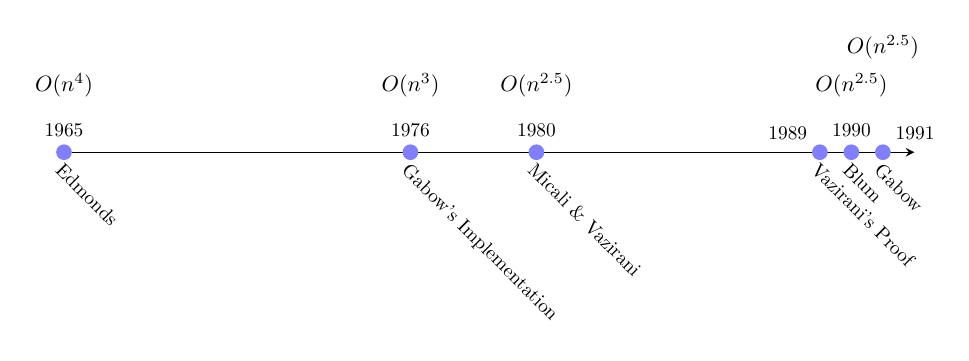
\begin{tikzpicture}[xscale=.4,every
    label/.style={scale=.7},>=stealth, on grid]
    \tikzstyle{node}=[circle, fill=blue!50, inner sep=2pt]
    \tikzstyle{aname}=[rotate=-45,scale=.7,anchor=north
    west]

    \node[node, label=above:1965] at (65,0) (ed) {};
    \draw[->] (ed) -- (92,0);
    \node[aname] at (ed) {Edmonds};
    \node[above=4ex,scale=.8] at (ed) {$O(n^4)$};

    \node[node, label=above:1976] at (76,0)
    (impl) {};
    \node[aname] at (impl) {Gabow's Implementation};
    \node[above=4ex,scale=.8] at (impl) {$O(n^3)$};

    \node[node, label=above:1980] at
    (80,0) (vaz) {};
    \node[aname] at (vaz) {Micali \& Vazirani};
    \node[above=4ex,scale=.8] at (vaz) {$O(n^{2.5})$};

    \node[node,label=above left:1989] at (89,0)
    (vazprf) {};
    \node[aname] at (vazprf) {Vazirani's Proof};

    \node[node, label=above:1990] at (90,0) (blum)
    {};
    \node[aname] at (blum) {Blum};
    \node[above=4ex,scale=.8,] at (blum) {$O(n^{2.5})$};

    \node[node, label=above right:1991] at (91,0) (gabow)
    {};
    \node[aname] at (gabow) {Gabow};
    \node[above=4ex,scale=.8,yshift=4ex] at (gabow) {$O(n^{2.5})$};
  \end{tikzpicture}
\end{frame}

\begin{frame} \frametitle{References}

  \begin{thebibliography}{1}
%      \bibitem{netflow00}
%    Rudolf Ahlswede, Ning Cai, Shuo-Yen~Robert Li, and
%    Raymond~W. Yeung.
    \bibitem{}
    Jack Edmonds
    \newblock Paths, {T}rees, and {F}lowers
    {\scriptsize \newblock {\em Canadian Journal of Mathematics},
      17:449--467, 1965.
      \url{http://www.cs.berkeley.edu/~christos/classics/edmonds.ps}}

    \bibitem{}
      Harold N. Gabow
      \newblock An {E}fficient {I}mplementation of {E}dmonds'
      {A}lgorithm for {M}aximum {M}atching on {G}raphs
      {\scriptsize \newblock {\em Journal of the ACM (JACM)},
      23(2):221--234, 1976.}
      
    \bibitem{}
      Norbert Blum
      \newblock A {N}ew {A}pproach to {M}aximum {M}atching in
      {G}eneral {G}raphs
      {\scriptsize \newblock {\em Lecture Notes in Computer Science:
          Automata, Languages and Programming},
        443::586--597, Springer Berlin / Heidelberg, 1990.}
  \end{thebibliography}
%   Combinatorial Optimization: Algorithms and Complexity
% By Christos H. Papadimitriou, Kenneth Steiglitz
% Contributor Kenneth Steiglitz
% Published by Courier Dover Publications, 1998
% ISBN 0486402584, 9780486402581
% 512 pages
\end{frame}

\begin{frame} \frametitle{Thank You}
  \begin{center}
    \Huge\bf\color{blue}
    Thank You!
  \end{center}
\end{frame}

\subsection{Questions}

\begin{frame} \frametitle{Questions}
  \begin{center}
    \Huge\bf\color{blue}
    {???}
  \end{center}
\end{frame}

\end{document}
